% Template for ICASSP-2018 paper; to be used with:
%          spconf.sty  - ICASSP/ICIP LaTeX style file, and
%          IEEEbib.bst - IEEE bibliography style file.
% --------------------------------------------------------------------------
\documentclass{article}
\usepackage{spconf,amsmath,amssymb,graphicx,bm,algorithm,algpseudocode,mathtools,xcolor}
\graphicspath{{figures/}}

% \newcommand{\R}{\mathbb{R}}
% \renewcommand{\vec}[1]{\ensuremath{\mathbf{#1}}}
% \providecommand{\mat}[1]{\ensuremath{\mathbf{#1}}}
% \providecommand{\vx}{\vec{x}}
% \providecommand{\vy}{\vec{y}}
% \providecommand{\ve}{\vec{e}}
% \providecommand{\vn}{\vec{n}}
% \providecommand{\vA}{\vec{A}}
\providecommand{\norm}[1]{\left\lVert#1\right\rVert}
\DeclareMathOperator*{\argmin}{arg\,min}
\DeclareMathOperator*{\argmax}{arg\,max}

\title{Optimal Measurement Configuration in Computational \\ Multispectral Imaging With a Diffractive Lens}

\name{Evan Widloski \qquad Ulas Kamaci \qquad Farzad Kamalabadi}
\address{
Department of Electrical and Computer Engineering and Coordinated Science Laboratory, \\
University of Illinois at Urbana-Champaign, Urbana, IL 61801, USA
}

\begin{document}
\maketitle

\begin{abstract}
% Spectral imaging, forming images of a scene at many wavelengths, is a
% fundamental analysis technique with many scientific applications. Diffractive
% lenses can achieve very high resolution in x-ray and UV regimes as compared to
% reflective and refractive optics. Their wavelength dependent focal length
% enables them to be used in spectral imaging of polychromatic sources, where the
% focused image of each spectral component is formed at different distances from
% the diffractive lens. If measurements are taken at each of these focus
% locations, it is possible to computationally reconstruct the spectral scene by
% solving an inverse problem. In this paper, we propose a greedy algorithm for
% finding a measurement configuration which results in better reconstructions than
% a conventional configuration selection strategy.

In this paper, we investigate the problem of data acquisition in a multispectral
diffractive imaging system.  Diffractive systems have the property that the
spectral components of a polychromatic source are focused at different distances
from the lens.  This means that in order to image a source at more than one
wavelength, multiple measurements must be made with a moving detector. However,
the choice of where to make these measurements is non-obvious and has
implications on the quality of the reconstructions. Furthermore, an exhaustive
search of all possible measurement configurations grows exponentially with the
number of sources and is computationally infeasible. We propose a greedy
backward elimination algorithm for finding acquisition locations and show that
reconstruction quality is improved over a naive acquisition strategy.
\end{abstract}

\begin{keywords}
Spectral imaging, diffractive optics, measurement configuration, sequential
backward selection, subset selection
\end{keywords}

\section{Introduction}
\label{sec:intro}
Spectral imaging is the formation of images at different wavelengths in the
electromagnetic spectrum.  With images usually taken in the visible, x-ray,
ultraviolet (UV), or infrared bands (IR), it has applications in medicine, geographic
surveying, astronomy, and solar physics.  Spectral imaging can be further broken
down into the categories of \emph{hyperspectral imaging} and \emph{multispectral imaging}.
Hyperspectral imaging is the capture of a scene over a contiguous spectrum,
while multispectral imaging is the capture of a set narrow, usually non-adjacent
bands of interest.  In both cases, a polychromatic source must be first
separated into its spectral components before being captured.  There are a
number of ways to achieve this, but a common method is to use a set of
configurable optical filters.  For example, the spectral imager on the Solar
Dynamics Observatory uses a rotating drum of optical filters to selectively pass
light of specific wavelengths of interest.

% Spectral imaging is forming images of a scene as a function of wavelength, is a
% fundamental diagnostic technique in various fields such as astronomy,
% surveillance, agriculture and medicine \cite{shaw2003spectral},
% \cite{garini2006spectral}. Forming a three dimensional (3D) data-cube (one
% wavelength and two spatial dimensions) with two dimensional (2D) detector
% measurements can be done by taking multiple exposures. To capture the spectrum
% of a scene, conventional spectral imagers combine regular camera optics with
% either additional wavelength filters or dispersive elements (e.g diffraction
% grating).

An alternative approach is to use a diffractive lens to perform spectral
imaging \cite{oktem2014icip}.  Diffractive lenses have the property that light at different
wavelengths will exit the lens at different angles, which has the effect of
creating a focused image of the light source at separate planes for each
spectral component of the source (Figure \ref{fig:diff_lens}(a)).

Diffractive lenses are often preferred in the UV or x-ray regimes over
reflective optics because manufacturing tolerances at these wavelengths must be
much tighter than in the visible regime in order to get a similar optical
performance.  Since diffractive optics can be manufactured using a
photolithographic process, they can be produced at a higher precision compared
to the grinding process used to produce conventional reflective optics.
Similarly, refractive optics are unsuitable for UV or x-ray imaging because
glass is opaque at these wavelengths. Figures \ref{fig:diff_lens}(b) and
\ref{fig:diff_lens}(c) are two examples of a pattern that can be etched into
silicon wafer to produce a diffractive lens.

\begin{figure}[htb]

\begin{minipage}[b]{0.48\linewidth}
  \centering
  \centerline{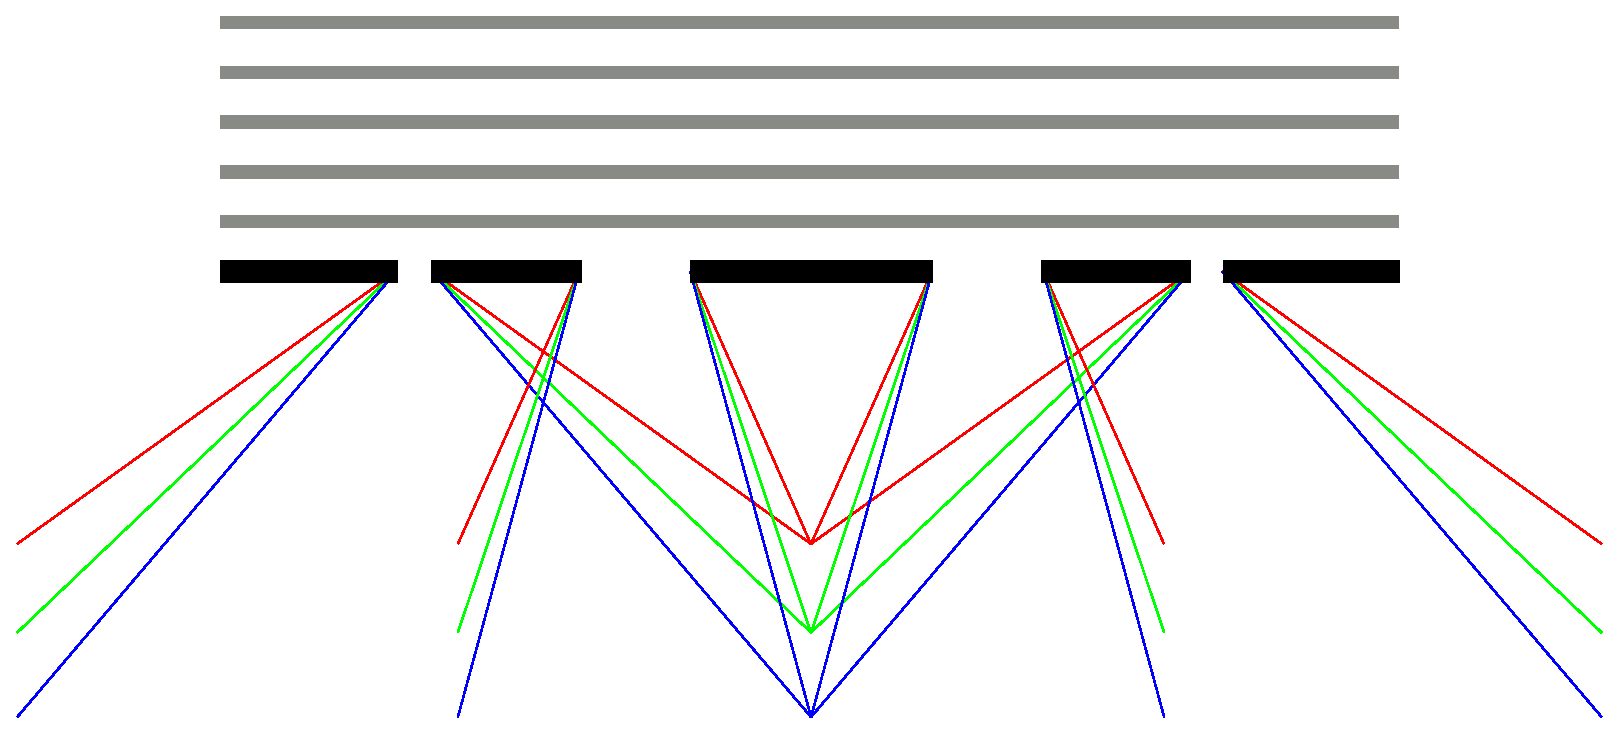
\includegraphics[width=4.0cm]{diffraction_ps_rgb}}
  \centerline{(a)}\medskip
\end{minipage}
\hfill
\begin{minipage}[b]{0.24\linewidth}
  \centering
  \centerline{
\includegraphics[width=2.0cm]{zoneplate}}
  \centerline{(b)}\medskip
\end{minipage}
\hfill
\begin{minipage}[b]{0.24\linewidth}
  \centering
  \centerline{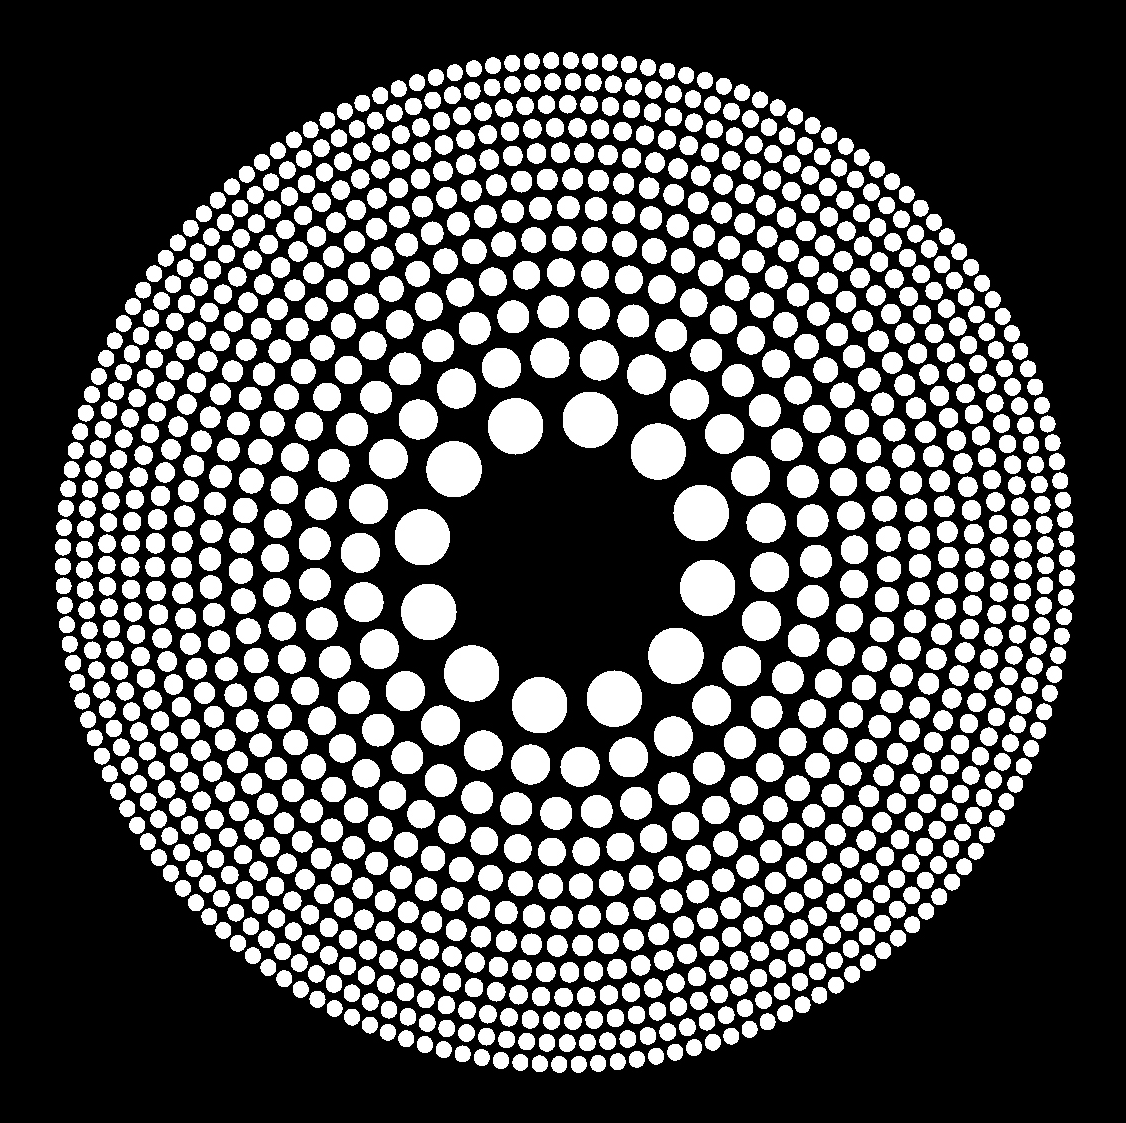
\includegraphics[width=2.0cm]{photonsieve}}
%  \vspace{1.5cm}
  \centerline{(c)}\medskip
\end{minipage}
\caption{(a) diffraction of a polychromatic wave through a diffractive lens (b) Fresnel zone
plate (c) photon sieve}
\label{fig:diff_lens}
%
\end{figure}

% FIXME
While diffraction produces a focused image of each source at separate planes, it
***.  This means that each measurement is actually a sum of all spectral
components of the source at varying degrees of focus.  An inverse problem
consisting of disentangling and deblurring of measurements must be solved in
order to recover the original source components.  Traditionally, measurement
locations are selected at the plane of focus for each spectral component.
However, as we show later in this paper, it is possible to improve on the
reconstruction quality in some situations by making measurements away from these
focal positions. We propose a greedy backward selection algorithm for
automatically discovering such a measurement configuration. Additionally, we
provide some bounds under which the greedy algorithm outperforms the traditional
selection approach.

% A different approach is to use a diffractive lens to perform spectral imaging.
% Diffractive lenses focus light using the diffraction principle. They have
% wavelength dependent focal length which is the property that enables them to be
% used as spectral imagers (see Figure \ref{fig:diff_lens}). Examples of
% diffractive lenses are Fresnel zone plates and their modifications (e.g. photon
% sieve) (see Figure \ref{fig:diff_lens}). Diffractive lenses are preferred in
% applications in UV and x-ray regimes where they can provide high resolution
% whereas reflective optics are very costly to manufacture to achieve high
% resolution and refractive lenses cannot be used due to light absorption in these
% regimes.


% Photon sieve spectral imaging (PSSI) is a modality that takes the advantage of
% the wavelength dependent focal length of a photon sieve to perform high
% resolution spectral imaging \cite{oktem2014icip}. It takes multiple exposures of
% the scene at different distances from the lens. Figure \ref{fig:pssi_drawing}
% illustrates the PSSI measurements for a scene radiating at two wavelengths
% $\lambda_1$ and $\lambda_2$. Each measurement consists of blurred superposition
% of the spectral images. The spectral images are then reconstructed from these
% measurements by solving a multi-frame deconvolution problem.


\begin{figure}[htb]
  \begin{minipage}[b]{1\linewidth}
    \centering
    \centerline{\includegraphics[width=8.5cm]{drawing}}
  \end{minipage}
  \caption{Imaging a scene with emissions at wavelengths $\lambda_1$ and
  $\lambda_2$. Measurements $y_1$ and $y_2$ are taken at two positions where one wavelength
  is in focus and the other is out of focus.}
  \label{fig:pssi_drawing}
\end{figure}

% Choice of measurement planes is an important factor affecting the reconstruction
% quality of the spectral images. Where to take measurements to maximize the
% fidelity of the reconstructions?

% One way is to scan the
% wavelength dimension by using color filters with narrow bandpass to filter
% desired wavelengths at each exposure. Another way is to capture the whole
% spectrum of a portion of the scene at an exposure, and scan a spatial dimension.
% In both methods, the 3D data-cube is then simply reconstructed by stacking the
% 2D measurements in the scanning dimension.

% There are also computational methods which rely on signal processing methods and
% computational power to improve upon the conventional methods in terms of spatial
% and spectral resolutions, total exposure time etc. They utilize more
% sophisticated image acquisition techniques than the conventional scanning-based
% methods, and computationally reconstruct the data-cube from multiplexed/encoded
% measurements. Such methods include compressive coded aperture snapshot spectral
% imaging (CASSI) [REF], compressive hyperspectral imaging by separable spectral
% and spatial operators (CHISS) [REF], and photon sieve spectral imaging (PSSI)
% \cite{oktem2014icip}.

% We will use PSSI as an example modality to explain and demonstrate our work
% because it  uses a diffractive lens, and it is a computational spectral imaging
% modality \cite{oktem2014icip}. Photon sieves, just like Fresnel zone plates, are
% diffractive lenses that use diffraction phenomenon to focus light. Diffractive
% lenses are preferred in applications in UV and x-ray regimes since they can
% provide high resolution whereas reflective optics are very costly to manufacture
% to achieve high resolution and refractive lenses cannot be used due to light
% absorption. They have wavelength dependent focal length which is what behind the
% working principle of PSSI. It takes multiple exposures at different distances
% from the lens to sample the measurement space.

\section{Forward Model and Statistical Formulation}
\label{sec:format}
In this section, we mathematically model a diffractive imaging
system and describe the process of recovering the spectral components. Consider
a polychromatic source that has $S$ two-dimensional spectral components
$\bm{x}_1, \dots, \bm{x}_S$. Using a moving detector, we make $M$
two-dimensional measurements $\bm{y}_1, \dots, \bm{y}_M$ at distances $d_1,
\dots, d_M$ from the lens. We allow for repeated measurements at the same plane
for a more flexible model that can take into account non equal exposure times.
% FIXME
Due to linearity, each measurement is a superposition of blurred versions
of the $S$ sources. More formally,

\begin{equation}
\bm{y}_m = \sum_{s=1}^S \bm{a}_{m,s} \ast \bm{x}_s + \bm{n}_s
\label{eq:fwd_model}
\end{equation}

where $\bm{a}_{m,s}$ is a blurring kernel known as a \emph{point spread
function} (PSF) and $\ast$ is a 2D circular convolution. Each PSF depends on the
associated source wavelength and measurement location and can be computed
analytically. An example set of PSF images for $M=S=2$ case is given in Figure
\ref{fig:psfs}.
% FIXME - explanation not technically correct


Since convolution is a linear operation, we can rewrite the above equation as a
linear system

\begin{equation}
  \underbrace{
    \begin{bmatrix}\bm{y}_1 \\ \vdots \\ \bm{y}_M\end{bmatrix}
  }_{\bm{y}}
  =
  \underbrace{
    \begin{bmatrix}
      \bm{A}_{1, 1} & \hdots & \bm{A}_{1, S} \\
      \vdots & & \vdots \\
      \bm{A}_{M, 1} & \hdots & \bm{A}_{M, S}
    \end{bmatrix}
  }_{\bm{A}_{\bm{d}}}
  \underbrace{
    \begin{bmatrix}\bm{x}_1 \\ \vdots \\ \bm{x}_S\end{bmatrix}
  }_{\bm{x}}
  +
  \underbrace{
    \begin{bmatrix}\bm{n}_1 \\ \vdots \\ \bm{n}_M\end{bmatrix}
  }_{\bm{n}}
\label{eq:fourier_mtx}
\end{equation}

\begin{figure}[htb]
  \begin{minipage}[b]{1\linewidth}
    \centering
    \centerline{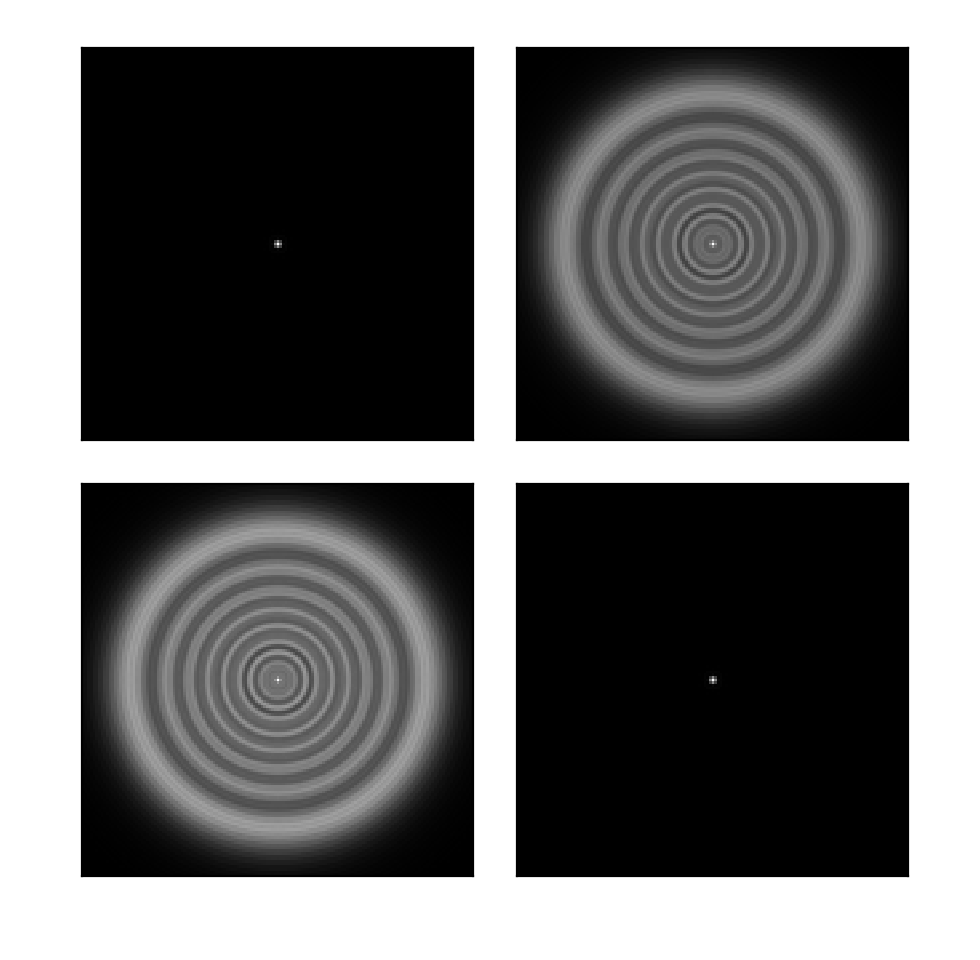
\includegraphics[width=5cm]{psfs}}
  \end{minipage}
  \caption{Example point spread functions for measuring a source with 2 spectral
    components at the focal planes of each component.}
  \label{fig:psfs}
\end{figure}

where $\bm{y}_m$, $\bm{x}_s$ and $\bm{n}_m$ have been flattened from their
original 2D shape, and each $\bm{A}_{m,s}$ is a block-circulant
matrix with circulant blocks (BCCB) formed from 2D convolution with PSF $\bm{a}_{m,s}$.
We will refer to the matrix containing all $\bm{A}_{m,s}$
generated by measurements taken at $\bm{d} = \{d_1, \dots, d_M\}$ as
$\bm{A}_{\bm{d}}$.

The problem of where to take measurements $\bm{y}_1, \dots, \bm{y}_M$ has not
been addressed and impacts the reconstruction quality.  In order to
compare the relative quality of different measurement configurations, it is
necessary to define some cost for the measurement matrix $\bm{A}_{\bm{d}}$.  A common cost
metric is the expected reconstruction error, or expected sum of squared errors
(SSE). However, we must have some strategy for the recovery of $\bm{x}$ to get
reconstruction error and we must make statistical assumptions about $\bm{x}$.
Maximum a posteriori (MAP) estimation is one such strategy.

We assume the original spectral components and noise are distributed according to a
normal distribution such that $\bm{x} \sim \mathcal{N}(\bm{\mu}_{\bm{x}}, \bm{\Sigma}_{\bm{x}})$ and
$\bm{n} \sim \mathcal{N}(0, \bm{\Sigma}_{\bm{n}})$.  The MAP estimate is then

% FIXME - dimensionality -> n
% use A instead of H?
$$
\begin{aligned}
  \bm{x}_{MAP} &= \arg \max_{\bm{x} \in \mathbb{C}^n} p(\bm{x} | \bm{y})
  = \arg \max_{\bm{x}} p(\bm{y}|\bm{x}) p(\bm{x})\\
  &= \arg \min_{\bm{x}} \left[  - \log(p(\bm{y}|\bm{x})) - \log
  p(\bm{x})\right] \\
  &= \bm{x}_0 + \left( \bm{A}_{\bm{d}}^H\bm{\Sigma}_{\bm{n}}^{-1} \bm{A}_{\bm{d}} +
    \bm{\Sigma}_{\bm{x}}^{-1}\right)^{-1}
  \cdot  \bm{A}_{\bm{d}}^H \bm{\Sigma}_{\bm{n}}^{-1} (\bm{y} - \bm{A}_{\bm{d}} \bm{\mu}_{\bm{x}})
\end{aligned}
$$
The reconstruction error is defined as $\bm{e} = \bm{x} - \bm{x_{\text{MAP}}}$,
and the expected sum of squared error cost is $E[\norm{\bm{e}}_2^2]$. This
expression can be rewritten in terms of the error covariance:

\begin{align*}
E[\norm{\bm{e}}_2^2] =  E[\bm{e}^H\bm{e}] & = E[tr(\bm{e}^H\bm{e})] = E[tr(\bm{e}\bm{e}^H)] \\
& = tr(E[\bm{e}\bm{e}^H]) = tr(\bm{\Sigma}_{\bm{e}})
\end{align*}

where the error covariance matrix is defined as $\bm{\Sigma}_{\bm{e}} =
E[\bm{e}\bm{e}^H]$ and has the closed form expression:
\begin{equation}
\bm{\Sigma}_{\bm{e}} = \left( \bm{A}_{\bm{d}}^H\bm{\Sigma}_{\bm{n}}^{-1} \bm{A}_{\bm{d}} +
    \bm{\Sigma}_{\bm{x}}^{-1}\right)^{-1}
\end{equation}

Combining the above equations, we can now write a cost metric which lets us evalute
the expected reconstruction error for a particular measurement configuration $\bm{d}$:
\begin{equation}
\text{Cost}(\bm{d}) = E[\norm{\bm{e}}_2^2] = tr\left(\left( \bm{A}_{\bm{d}}^H\bm{\Sigma}_{\bm{n}}^{-1} \bm{A}_{\bm{d}} +
    \bm{\Sigma}_{\bm{x}}^{-1}\right)^{-1}\right)
\end{equation}

% In this section, we mathematically model a multispectral diffractive imaging system.
% Consider a polychromatic source that has spectral emissions at $S$ distinct
% wavelengths $\lambda_1, \dots, \lambda_S$. Using a moving detector,
% we take measurements at $M$ different measurement planes, with distances from the
% sieve $d_1, \dots, d_M$ (see Figure \ref{fig:meas}).  Each of these $M$
% measurements is a sum over the $S$ sources, with each source blurred to varying
% degrees.

% With this,
% the discrete model that relates the noiseless measurements to the sources is
% given by the following model:
% \begin{equation}
% y_k[m,n] = \sum_{p=1}^P h_{d_k,\lambda_p}[m,n] \ast x_p[m,n] \ , \ k = 1,2,\dots, K
% \label{eq:fwd}
% \end{equation}
% where $m,n=-N/2, \dots, N/2-1$ assuming that the detector has $N\times N$
% pixels. Here, $x_p$ denotes the discretized intensity of the source with
% wavelength $\lambda_p$, and $h_{d_k,\lambda_p}$ denotes the discretized point
% spread function (PSF) of the photon sieve for the wavelength $\lambda_p$ and
% plane distance $d_k$, which has a closed form expression given in
% \cite{oktem2013icip}. So, each measurement $y_k$ is a superposition of all the
% sources $x_p$ convolved with their corresponding PSFs $h_{d_k,\lambda_p}$.

% \begin{figure}[h]
% 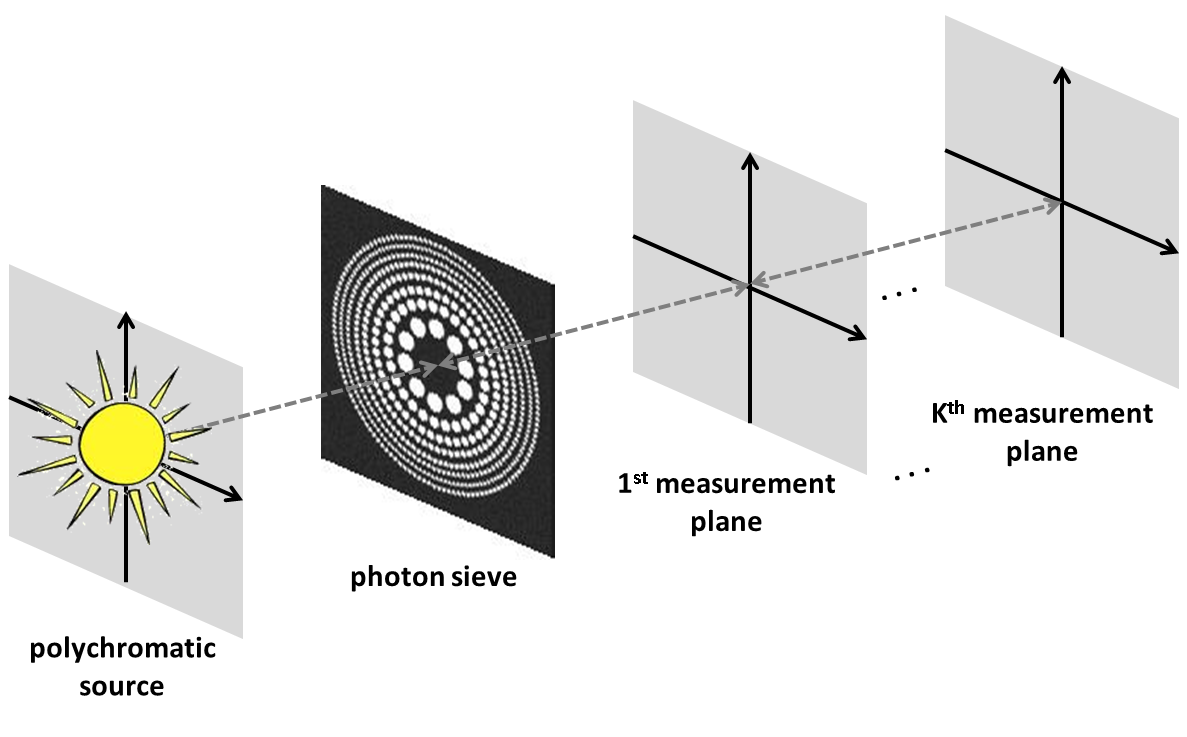
\includegraphics[width=0.45\textwidth]{poster1}
% \caption{PSSI measurement configuration.}
% \label{fig:meas}
% \end{figure}


% Since \eqref{eq:fwd} is a linear relation between the sources and the
% measurements, we can represent it using matrix-vector form which will be useful
% in formulating the inverse problem. Denote by $\vx_p$ and $\vy_k$ the vectorized
% versions of $x_p[m,n]$ and $y_k[m,n]$. Then, we have
% \begin{equation}
% \vy = \vec A \vx + \vec w
% \label{eq:mtx-vec}
% \end{equation}
% with
% \begin{equation}
% \vy = \begin{bmatrix}
% \vy_1 \\ \vdots \\ \vy_K
% \end{bmatrix}, \vA = \begin{bmatrix}
% \vA_{11} \hspace{-.1 in}& \dots \hspace{-.1 in}& \vA_{1P} \\
% \vdots \hspace{-.1 in}& \ddots \hspace{-.1 in}& \vdots \\
% \vA_{K1} \hspace{-.1 in}& \dots \hspace{-.1 in}& \vA_{KP}
% \end{bmatrix}, \vx = \begin{bmatrix}
% \vx_1 \\ \vdots \\ \vx_P
% \end{bmatrix}, \vw = \begin{bmatrix}
% \vw_1 \\ \vdots \\ \vw_K
% \end{bmatrix}
% \end{equation}

% where $\vw_k \in \R^{N^2}$ is additive Gaussian noise vector with $(\vw_k)_i
% \sim \mathcal N (0, \sigma_k^2)$; and $\vA_{k,p} \in \R^{N^2 \times N^2}$ is the
% convolution matrix corresponding to the PSF $h_{d_k,\lambda_p}$. We assume that
% the periodic boundary conditions hold, which makes the matrices $\vA_{k,p}$
% block circulant with circulant blocks (BCCB). This allows computationally
% efficient algorithms in the image reconstruction.


\section{Measurement Selection Algorithm}

With a method of evaluating the effect a particular configuration $\bm{d}$ has
on reconstruction error, we can begin considering which configurations are best
suited for minimizing error.  For example, if we are provided with a set of $C$
candidate measurement locations, we may wish to find a subset of size $M$ which
minimizes reconstruction error. This is known as a \emph{subset selection} problem.
One might think to simply  search over all possible measurement configurations
of size $M$, but this exhaustive search requires $\binom{C}{M}$ evalutions of
cost, growing on the order of $O(C^M)$.
% With a method of comparing the *** of two measurement configurations, one might
% think to simply search all possible measurements and choose the best.  However,
% the computational cost of an exhaustive search grows too quickly and is
% infeasible for most realistic scenarios.  For example, consider a scenario in
% which there are $C$ candidate measurement locations of which we would like to
% select a subset of size $M$ to form our measurement matrix $\bm{A}$.
% Exhaustively searching through all possible configurations of $\bm{A}$ would
% require $\binom{C}{M}$ iterations, recomputing $\text{Cost}(\bm{A})$ each time.

An alternative method which is more computationally feasible is known as
\emph{greedy hill climbing}, or more specifically, \emph{sequential backward
selection} (SBS) \cite{sharif}. In SBS, one measurement location is eliminated from $\bm{d}$ in each
iteration until only $M$ locations remain. As reconstruction error generally
increases as the number of measurements dereases, SBS selects for elimination the
measurement that incurs the smallest increase in cost in each iteration.

\begin{algorithm}
  \begin{algorithmic}
    \caption{SBS Algorithm}
    \State $\bm{d} = \{d_1, \dots, d_C\}$
    \Repeat
      \State $d' = \arg \min_{d \in \bm{d}} \text{Cost}(\bm{d} \backslash d))$
      \State $\bm{d} = \bm{d} \backslash d'$
    \Until{$|\bm{d}| = M$}
  \end{algorithmic}
\end{algorithm}

Unlike an exhaustive search, the complexity of SBS is not combinatorial.  As the
size of $\bm{d}$ shrinks with each iteration, the number of cost evaluations for each
minimization step decreases.  The total number of cost evaluations is

$$
\begin{aligned}
  \sum_{|\bm{d}| = M}^C |\bm{d}|
  &= \frac{C
    (C + 1)}{2} - \frac{M(M + 1)}{2} \\
  &= O(C^2 - M^2)
\end{aligned}
$$

% Having defined the cost metric, we are now looking for the best measurement
% configuration to minimize the cost. Suppose we take $M$ measurements, each at
% a distance $d_m$ from the lens for $m = 1, \dots, M$.

% \begin{equation}
% \hat {\bm A} = \argmin_{\vA \in Q} \ \text{Cost}(\bm{A})
% \label{eq:inverse}
% \end{equation}
% The goal in the inverse problem is to reconstruct the spectral components
% $\bm{x}_1, \dots, \bm{x}_S$ from the noisy, blurry and superimposed measurements
% $\bm{y}_1, \dots, \bm{y}_M$. This is known as a \emph{multi-frame deconvolution
% problem} with multiple sources.  However, deconvolution is known to be highly
% ill-posed, which means that direct inversion of the matrix containing the PSFs
% (or its least square approximation) amplifies the noise in the measurements and
% leads to poor reconstructions. To avoid noise amplification, the problem needs
% to be regularized. The inverse problem can then be formulated as a regularized
% optimization problem as follows:
% \begin{equation}
% \hat \vx = \argmin_{\vx} \norm{\vA\vx-\vy}_2^2 + \lambda \mathcal R(\vx)
% \label{eq:inverse}
% \end{equation}
% where the first term ensures that the reconstructions comply with the
% measurements and the second term is the regularization term with parameter
% $\lambda>0$. In this paper, we are interested in

\section{Fast Implementation}
Computational complexity of the algorithm can be significantly reduced by
exploiting the BCCB structure of the blocks of $\bm {A_d}$ together with
assuming the same structure in $\bm {\Sigma_n}$ and $\bm {\Sigma_x}$. We assume
that each candidate plane has the same noise level with noise variance
$\sigma^2$ uncorrelated among all pixels, so $\bm {\Sigma_n} = \sigma^2 \bm
I_{CN^2}$ where $\bm I_{CN^2}$ is an identity matrix of dimension $CN^2$. We
also assume that $\bm {\Sigma_{x}}^{-1}= \alpha \bm D ^T \bm D \in \mathbb
R^{SN^2 \times SN^2}$ where $\bm D =\bm I_S \otimes \bm D_0 $ consists of BCCB
blocks, $\bm D_0 \in \mathbb R^{N^2 \times N^2}$, which for example could
correspond to a high pass filter for globally smooth signal prior.

Having set the assumptions, let's now see how we exploit the BCCB structures.
Note that BCCB matrices can be diagonalized by the 2D DFT matrix, hence, each
$N^2 \times N^2$ block $\bm A_{c,s}$ of $\bm {A_d}$ can be decomposed as $\bm
A_{c,s} = \bm F^{-1} \widetilde{\bm A}_{c,s} \bm F$ where $\widetilde{\bm
A}_{c,s}$ is diagonal. This yields
\vspace{-0.1 in}
\begin{equation}
  \bm {A_d}=
  \underbrace{
    \begin{bmatrix}
      \bm F^{-1} \hspace{-0.2 in}& \hspace{-0.2 in} & \hspace{-0.1 in} \vspace{-0.1 in}\text{\Large 0} \\
        \vspace{-0.05 in}& \ddots &  \\
      \text{\Large 0} \hspace{-0.1 in}& \hspace{-0.2 in} & \hspace{-0.2 in} \bm F^{-1}
    \end{bmatrix}
  }_{\widetilde{\bm F}^{-1}}
  \underbrace{
    \begin{bmatrix}
      \widetilde{\bm A}_{1,1} \hspace{-0.1 in}& \hdots & \hspace{-0.1 in} \widetilde{\bm A}_{1,S} \vspace{-0.02 in}\\
      \vspace{-0.02 in}\vdots & & \vdots \\
      \widetilde{\bm A}_{M,1} \hspace{-0.1 in}& \hdots & \hspace{-0.1 in} \widetilde{\bm A}_{M,S} \\
    \end{bmatrix}
  }_{\widetilde{\bm A}_{\bm d}}
  \underbrace{
    \begin{bmatrix}
      \bm F \hspace{-0.1 in}& \hspace{-0.2 in} & \hspace{-0.1 in} \vspace{-0.1 in}\text{\Large 0} \\
        \vspace{-0.05 in}& \ddots &  \\
      \text{\Large 0} \hspace{-0.1 in}& \hspace{-0.2 in} & \hspace{-0.2 in} \bm F
    \end{bmatrix}
  }_{\widetilde{\bm F}}
\label{eq:fourier_mtx}
\end{equation}
\vspace{-0.1 in}

% $\bm {A_d} = (\bm I_C \otimes \bm F^{-1}) \bm {\Gamma_d} (\bm I_S \otimes \bm
% F)$, where $\bm {\Gamma_d} \in \mathbb R^{CN^2 \times SN^2}$ has the diagonal
% blocks $\bm \Gamma_{c,s}$.

so, we have $\bm{A_d} = \widetilde{\bm F}^{-1} \widetilde{\bm A}_{\bm d}
\widetilde{\bm F}$, from which we get $\bm{A_d}^H \bm{A_d} = \widetilde{\bm
F}^{-1} \widetilde{\bm A}_{\bm d}^H \widetilde{\bm A}_{\bm d} \widetilde{\bm
F}$. Applying the same procedure to the other term, we get $\bm D^H \bm D =
\widetilde{\bm F}^{-1} \widetilde{\bm D}^H \widetilde{\bm D} \widetilde{\bm F}$.
The SSE cost then becomes:
\begin{align}
\text{Cost}(\bm{d}) & = tr\left(\left(
{\bm A}_{\bm d}^H {\bm A}_{\bm d} + \lambda {\bm D}^H
{\bm D} \right)^{-1} \right)
\label{eq:naive_cost}\\
& = tr\left(\left(\widetilde{\bm F}^{-1} \widetilde{\bm
A}_{\bm d}^H \widetilde{\bm A}_{\bm d} \widetilde{\bm F} + \lambda \widetilde{\bm
F}^{-1} \widetilde{\bm D}^H \widetilde{\bm D} \widetilde{\bm
F}\right)^{-1}\right) \nonumber \\
& = tr\left(\left(\widetilde{\bm F}^{-1} \left(
\widetilde{\bm A}_{\bm d}^H \widetilde{\bm A}_{\bm d} + \lambda \widetilde{\bm D}^H
\widetilde{\bm D} \right) \widetilde{\bm F}\right)^{-1}\right) \nonumber \\
& = tr\left(\widetilde{\bm F}^{-1} \left(
\widetilde{\bm A}_{\bm d}^H \widetilde{\bm A}_{\bm d} + \lambda \widetilde{\bm D}^H
\widetilde{\bm D} \right)^{-1} \widetilde{\bm F}\right) \nonumber \\
& = tr\left(\left(
\widetilde{\bm A}_{\bm d}^H \widetilde{\bm A}_{\bm d} + \lambda \widetilde{\bm D}^H
\widetilde{\bm D} \right)^{-1} \right)
\label{eq:fast_cost}
\end{align}
where the computational complexity of \eqref{eq:fast_cost} is much less than
\eqref{eq:naive_cost} as both the multiplication and the inversion cost reduces
significantly due to the diagonalized blocks.

\section{Complexity Analysis}

\subsection{Naive Implementation}

The computational complexity of evaluating cost for a particular measurement
configuration $\bm{d}$ comes from two places in the cost formulation.

$$
  \text{Cost}(\bm{d}) = \text{tr} \Bigl(
  \overbrace{\vphantom{\rule[1.5em]{0pt}{0pt}}
(\underbrace{\vphantom{\rule[-0.5em]{0pt}{0pt}} \bm{A}_{\bm{d}}^H \bm{A}_{\bm{d}}}_{O_m}
-\lambda \bm{D}^H\bm{D})^{-1}
}^{O_i}
\Bigr)
$$

The first contributor to cost complexity is the multiplication of
$\bm{A}^H_{\bm{d}}\bm{A}_{\bm{d}}$.
Since the number of rows of $\bm{A}_{\bm{d}}$ varies with iteration, the
multiplication cost complexity varies with $|\bm{d}|$.
We denote this as $O_m(|\bm{d}|)$.  $\bm{A}_{\bm{d}}$ has shape $(|\bm{d}|N^2
\times SN^2)$, so complexity is

$$O_m(|\bm{d}|) = O\big( (SN^2)^2 \cdot |\bm{d}| N^2\big) = O(S^2N^6 |\bm{d}|)$$

As the dimensions of $\bm{A}^H_{\bm{d}} \bm{A}_{\bm{d}}$ and $\bm{D}^H \bm{D}$
do not depend on $\bm{d}$, the complexity of inversion in each cost computation
is fixed and does not vary with SBS iteration.  We call this $O_i$.

$$O_i = O\big( (SN^2)^3 \big) = O(S^3N^6)$$

The complexity of evaluating cost is $O_m(|\bm{d}|) + O_i$, and since the minimization step of SBS requires $|\bm{d}|$ evaluations of cost, the
overall complexity of the algorithm is

\begin{align*}
  O_{sbs} &= \sum_{|\bm{d}| = M}^C |\bm{d}| \Big( O_m(|\bm{d}|) + O_i \Big) \\
  &= \sum_{|\bm{d}| = M}^C O(S^2N^6|\bm{d}|^2) + \sum_{|\bm{d}| = M}^C O(S^3N^6|\bm{d}|) \\
  &= \underbrace{O(S^2N^6C^3)}_{\text{multiplication complexity}} + \underbrace{O(S^3N^6C^2)}_{\text{inversion complexity}}
\end{align*}

where we assume $C \gg M$ and use the fact that

$\sum_{|\bm{d}| =M}^C O(|\bm{d}|^2) = O(C^3)$ and

$\sum_{|\bm{d}| = M}^C O(|\bm{d}|)= O(C^2)$.

\subsection{Fast Implementation}

$$
\text{Cost}(\bm{d}) = tr\left(\left(
\widetilde{\bm A}_{\bm d}^H \widetilde{\bm A}_{\bm d} + \lambda \widetilde{\bm D}^H
\widetilde{\bm D} \right)^{-1} \right)
$$

$$
\bm{A}^H_{\bm{d}} \bm{A}_{\bm{d}} = \sum_{d \in \bm{d}} \bm{A}^H_{d} \bm{A}_{d}
$$

As mentioned previously, $\widetilde{\bm{A}}^H_{\bm{d}} \widetilde{\bm{A}}_{\bm{d}}$ can be formed by
summation of all $\bm{A}^H_d \widetilde{\bm{A}}_d$. Since each $\bm{A}_d$ has shape $(1
\times S)$ with diagonal blocks of size $N^2$, the overall complexity for
precomputing $\bm{A}^H_d \bm{A}_d$ for all $C$ candidate locations is

$$
O_m = C \cdot O(S^2N^2) = O(S^2N^2C)
$$

$O_m$ now refers to the complexity of the precomputed multiplication step, which
does not depend on $|\bm{d}|$ and occurs in algorithm initialization.
Similarly, the complexity of inversion decreases due to the diagonal blocks of
$\bm{A}^h_{\bm{d}} \bm{A}_{\bm{d}}$ and $\bm{D}^H \bm{D}$.

$$
O_i = O(S^3N^2)
$$

\begin{align*}
  O_{sbs} &= O_m + \sum_{|\bm{d}| = M}^C |\bm{d}| O_i = O(S^2N^2C) + \sum_{|\bm{d}| = M}^C O(S^3N^2|\bm{d}|) \\
  &= \underbrace{O(S^2N^2C)}_{\text{multiplication complexity}} + \underbrace{O(S^3N^2C^2)}_{\text{inversion complexity}}
\end{align*}

\section{Numerical Experiments}
\begin{itemize}
\item Describe the application with parameters (wavelengths, required resolution, sieve parameters, focal lengths, noise level, total exposure time limit, simulated images of sources). Justify the choices.

\item Describe the algorithm parameters (candidate plane locations, desired number of measurement planes, regularization parameter lambda, prior covariance matrix). Justify the choices.

\item Show the found CSBS planes together with the reconstruction results using these planes. Compare the CSBS reconstructions with the focal plane reconstructions. Interpret the results.

\item Discuss about under which conditions CSBS can outperform focal planes.
\end{itemize}

% Below is an example of how to insert images. Delete the ``\vspace'' line,
% uncomment the preceding line ``\centerline...'' and replace ``imageX.ps''
% with a suitable PostScript file name.
% -------------------------------------------------------------------------


\vfill\pagebreak

% References should be produced using the bibtex program from suitable
% BiBTeX files (here: strings, refs, manuals). The IEEEbib.bst bibliography
% style file from IEEE produces unsorted bibliography list.
% -------------------------------------------------------------------------
\bibliographystyle{IEEEbib}
\bibliography{bibliography}

\end{document}
